\section{Motivation}
\begin{figure*}[t]
	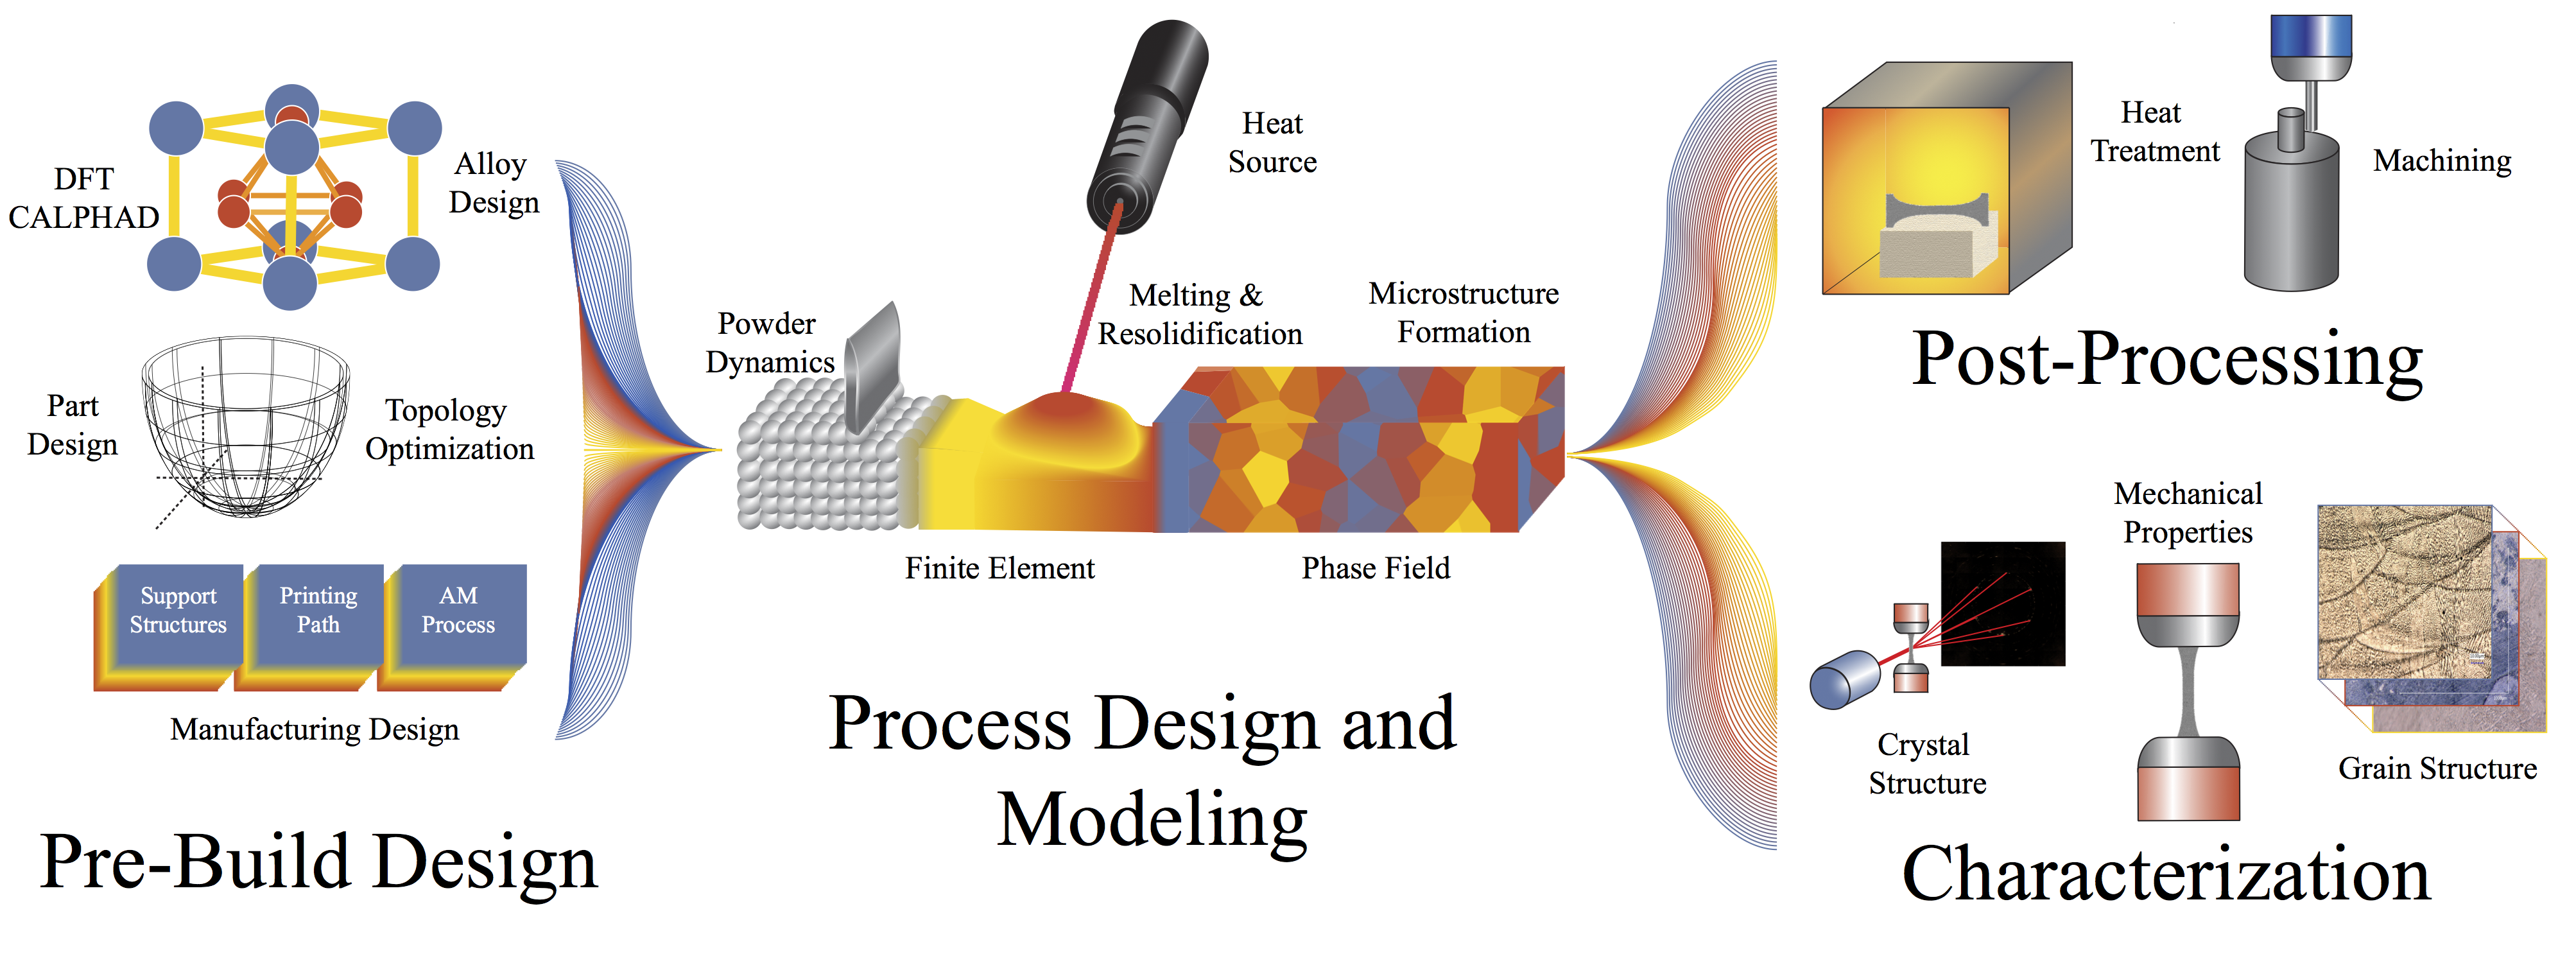
\includegraphics[width=1\linewidth]{Images/AMgene.png}
	\caption{Caption here}
	\label{AMgene}
\end{figure*}

Metals-based additive manufacturing (AM) represents a paradigm shift in how products are manufactured, providing versatility in the type and design of parts produced by a single manufacturing facility, decentralizing manufacturing capability, and enabling novelty in the properties and design of the parts, to name but a few benefits AM offers. However, there have been significant roadblocks to fully realize AM's potential, particularly in the control of consistency and quality in part production and in the development of materials amenable to the AM process. Although decades of immense scientific and engineering work in industry, academia, and government have produced large advances in making AM a practical manufacturing solution, the metallurgical challenges facing AM persist. Computational materials simulation and the Integrated Computational Materials Engineering (ICME) approach have made strides in accelerating materials development. The ICME approach for AM incorporates investigations across many fields and scientific methods. The wide, diverse array of promises and problems in AM has resulted in a field of study which is rich with data. In this paper, we argue that data-driven, statistically-based machine learning can complement and accelerate the ICME process for additive manufacturing. 


The 20th century saw the maturation of materials science and engineering as a field of study, enabling more rapid development of novel materials and materials manufacturing methods for specific applications. The process-structure-properties-performance paradigm transformed the combinatorial trial-and-error and intuition-driven materials discovery process into a problem of engineering a desired microstructure through designed processing. For instance, the history of turbine blade superalloy development is typified by advancements in control over microstructure through processing, including increasingly complex alloying recipes, multi-step heat treatments, and single-crystal casting. 

In the past decades, materials development has greatly accelerated to match the broader acceleration of general technology advancement. Computational materials science has enabled the prediction of microstructure from processing and of properties from microstructure, reducing the need for costly and time consuming experimentation. The Integrated Computational Materials Engineering (ICME) approach tightly integrates physics-based computational models into the industrial design process, allowing the desired performance requirements of a part to guide the design of a novel material. Examples include low-RE Ni superalloys for better turbine performance \cite{Pollock2016} and lower cost and the Ferrium S53 alloy designed for corrosion-resistant landing gears \cite{Olson2014}. Both cases took materials development timelines from decades to years, demonstrating the practical capability of designing new materials within an industrial product timeframe. Generalizing this capability to more industries and further accelerating the process is the primary goal of the Materials Genome Initiative (MGI) \cite{MGI}.

Current AM capabilities are limited by materials-based problems which are uniquely difficult to solve with the above paradigm. The AM process itself is complex relative to traditional casting methods, including rapid solidification, vaporization and ingestion of volatile elements, and a complex thermal history, all of which vary with part location and require advanced computational tools to properly predict microstructure and properties. However, the lower cost and time barrier to entry for performing AM has enabled the rapid accumulation of experimental data, enabling a high-throughput approach for finding optimized AM processing methods and parameters of existing alloys. For AM, the ICME-based tools have been catching up, attempting to bootstrap legacy models to this data, with limited success. As such, current AM materials development is largely combinatorial, as the processing of legacy alloys are optimized with extensive design of experiments and AM-specific alloys with higher performance are just now being effectively developed.

It is within this context we argue that machine learning (ML) can accelerate the application of additive manufacturing. ML as a method for model development has shown wide application in the past years, in industries ranging from finance \cite{Bose2001}, molecule design for chemistry and pharmacology \cite{Gomez-Bombarelli2018}, social networking \cite{Brusilovsky2007} and, most importantly to this review, materials science. The use of ML in materials has been relatively limited for a variety of reasons, primarily the lack of a curated and large dataset on which ML can operate. The MGI identified this as a primary problem for accelerating materials development, and there has been significant progress recently in infrastructure development for materials databases suitable for informatics tools such as ML. The difficulty in producing physics-based ICME models and the ability to rapidly and efficiently sample processing space in a combinatorial approach makes additive manufacturing an attractive use case for ML. Machine learning as a framework can couple legacy ICME tools with experimental data to produce much more accurate AM process-structure-property models and to automate the iteration of designed experiments for model improvement and optimized materials.

In this paper, we present our arguments for the use of ML to address AM challenges. We begin by phrasing terms and ideas from additive manufacturing in ways that are compatible with machine learning. We provide basics of machine learning algorithms and how they can be interpreted in an additive manufacturing study. Following this, we review machine learning methods that have been used in materials science previously. We attempt to state the uses of machine learning algorithms for addressing problems specific to additive. Following this, we cover the use of machine learning in materials science previously. We conclude with an outlook for how database-driven design of materials for AM can accelerate material creation and part qualification.
